\section{The modes of the finite walk}\label{sec:shape}

In this section and Appendices~\ref{app:shape} and~\ref{app:bulk},
``Assume~\eqref{eq:H}'' means
\begin{equation}\label{eq:H}
 N\ge64,\qquad0<\varepsilon\le\tfrac14,\qquad x=N\varepsilon\ge1 .\tag{H}
\end{equation}
We invoke this condition only where stated.
Recall that $P_N(N-m)=\frac12[f_N(m)+f_N(N-m)]$. For a mode $\kappa_N\ge N/2$ of $P_N$ we put $m_N=N-\kappa_N$, and $m_{\max}$ is the largest
mode of $f_N$.

\subsection{Families and the first flip}

\begin{figure}[t]
\centering
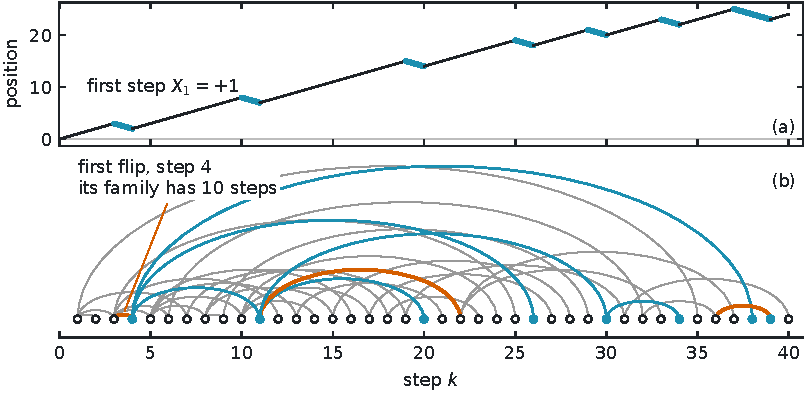
\includegraphics[width=\textwidth]{figures/Fig1}
\caption{One elephant walk with $N=40$ steps and $\varepsilon=0.07$. (a) The position against
the step. The steps that disagree with the first step are drawn heavier. (b) The memory tree of
the same walk. Step $k+1$ copies the step at the left end of its arc, and the arcs drawn heavier
are flips. A step disagrees with the first step exactly when the path from it to step $1$
crosses an odd number of flips (Lemma~\ref{lem:tree}). The first flip, at step $4$, turns its
family of ten steps. The flip at step $22$, inside that family, turns its own family of three
steps back, and the flip at step $39$ turns only that step.}
\label{fig:family}
\end{figure}

For $k_0\ge1$, the chain $(M^{[k_0]}_k)_{k\ge k_0}$ starts at
$M^{[k_0]}_{k_0}=0$ with transitions $r_k(b)$. It counts disagreeing steps when the first $k_0$ steps are forced
to agree. Thus $M^{[1]}$ has the law of $M$. Put $Y_d=M^{[1]}_d$ and $Z^{(j)}_t=M^{[j-1]}_t$ for
$j\ge2$, $t\ge j-1$. In a random recursive tree on $[N]=\{1,\dots,N\}$,
vertex $k+1$ joins a uniform vertex of $[k]$, independently for
$k=1,\dots,N-1$. The family $\mathcal T_v$ consists of $v$ and all its descendants.

\begin{lemma}[the memory tree]\label{lem:tree}
Let $\mathcal T$ be the tree on $[N]$ in which the parent of $k+1$ is $U_k$.
For $2\le v\le N$ let $\mu_v=1$ if step $v$ flips the step it copies, and
$\mu_v=0$ otherwise. Then $\mathcal T$ is a random recursive tree, the marks
$\mu_v$ are i.i.d.\ Bernoulli$(\varepsilon)$ and independent of $\mathcal T$,
and $X_v=X_1(-1)^{\sigma(v)}$, where $\sigma(v)$ is the number of marks on the
path from $v$ to the root, the root excluded. So $M_N=\#\{v:\sigma(v)\text{
odd}\}$. If the marks on $2,\dots,k_0$ are set to $0$, then the number of odd
vertices in $[k]$, $k\ge k_0$, is a copy of the chain $M^{[k_0]}$.
\end{lemma}

\begin{proof}
The parent $U_k$ of $k+1$ is uniform on $[k]$ and independent of the earlier
choices, and the marks are the flip indicators. The path from $k+1$ to the
root is $k+1$ followed by the path from $U_k$, so
$\sigma(k+1)=\mu_{k+1}+\sigma(U_k)$ and, by induction on $k$,
$X_{k+1}=X_{U_k}(-1)^{\mu_{k+1}}=X_1(-1)^{\sigma(k+1)}$. Now set
$\mu_2=\dots=\mu_{k_0}=0$. If $b$ of the vertices in $[k]$ are odd, $k\ge k_0$,
then $k+1$ is odd with conditional probability $(1-\varepsilon)\frac
bk+\varepsilon(1-\frac bk)=r_k(b)$, whatever else is known about $[k]$.
\end{proof}

A single flip at $v$ turns its family (Figure~\ref{fig:family}). For
$k\ge v$, a family $\mathcal T_v$ containing $s$ vertices of $[k]$
gains vertex $k+1$ with probability $s/k$. Lemma~\ref{lem:urn} gives
$\lvert\mathcal T_v\rvert$ law $\beta_v$, mean $N/v$, and an average
$N/(d(d+1))$ families of size $d$. If $v$ alone is marked,
$\mathcal T_v$ is the odd set. At fixed $N$, multiple marks have
probability $O(\varepsilon^2)$ and no mark gives $M_N=0$. Thus the
first-order part of $f_N(m)$ in $\varepsilon$ is
$\varepsilon\sum_v\beta_v(m)=x/(m(m+1))$ for $1\le m\le N-1$. This is \cite[Eq.~(10)]{bhs2023} with one
initial cell, and it is also proved in Lean for $M$
(Section~\ref{sec:verify}).

To go beyond first order we cut the tree at the first flip.

\begin{lemma}[splitting off a family]\label{lem:split}
Let $\mathcal T$ be a random recursive tree on $[N]$, let $2\le v\le N$ and
let $S\subseteq[N]$ with $\min S=v$. Given that $\mathcal T_v$ has vertex set
$S$, the restrictions of $\mathcal T$ to $S$ and to $[N]\setminus S$,
relabeled in increasing order, are independent random recursive trees. They
are independent of the parent of $v$, which is uniform on $[v-1]$.
\end{lemma}

\begin{proof}
The tree $\mathcal T$ is uniform over the $(N-1)!$ increasing trees on $[N]$.
Its family $\mathcal T_v$ has vertex set $S$ exactly when every $u\in
S\setminus\{v\}$ has its parent in $S$ and every $u\notin S$ with $u\ge2$ has
its parent outside $S$. So, given this event, each element of $S$ other than
$v$ picks its parent freely among the smaller elements of $S$, $v$ picks any
element of $[v-1]$, and each element of $[N]\setminus S$ other than $1$ picks
freely among the smaller elements of $[N]\setminus S$. This is the claim.
\end{proof}

\begin{lemma}[the first flip]\label{lem:firstmark}
Let $V=\min\{v\ge2:\mu_v=1\}$, with $V=\infty$ and $\lvert\mathcal T_V\rvert=0$ if there is no mark. If
$V<\infty$, let $\bar Y$ be the number of vertices $u$ of $\mathcal T_V$ with $\sigma(u)$ even, and
let $\bar Z$ be the number of odd vertices outside $\mathcal T_V$. Then for $2\le j\le N$,
$1\le d\le N-j+1$ and integers $y,z$,
\[
 \Prob\bigl(V=j,\,\lvert\mathcal T_V\rvert=d,\,\bar Y=y,\,\bar Z=z\bigr)
 =\varepsilon(1-\varepsilon)^{j-2}\beta_j(d)\,\Prob(Y_d=y)\,\Prob\bigl(Z^{(j)}_{N-d}=z\bigr).
\]
In particular $\Prob(V=j,\,\lvert\mathcal T_V\rvert=d)=\varepsilon(1-\varepsilon)^{j-2}\beta_j(d)$, and for $m\ge1$
\[
 f_N(m)=\sum_{j=2}^N\varepsilon(1-\varepsilon)^{j-2}\sum_{d=1}^{N-j+1}
 \beta_j(d)\,\Prob\bigl(d-Y_d+Z^{(j)}_{N-d}=m\bigr),
\]
where $Y_d$ and $Z^{(j)}_{N-d}$ are independent.
\end{lemma}

\begin{proof}
Marks and tree are independent, and $\lvert\mathcal T_j\rvert$ has the law $\beta_j$, which gives
the law of $(V,\lvert\mathcal T_V\rvert)$. Condition on
$V=j$ and on the vertex set $S$ of $\mathcal T_j$, with $\lvert S\rvert=d$.
The marks on $j+1,\dots,N$ are still i.i.d., and by Lemma~\ref{lem:split} the
trees on $S$ and on $[N]\setminus S$ are independent random recursive trees.
The vertices $1,\dots,j-1$ carry no mark, so $j$ is odd, and $u\in S$ is even
exactly when the path from $u$ up to $j$, with $j$ excluded, has an odd
number of marks. So by Lemma~\ref{lem:tree} for the tree on $S$ rooted at
$j$, the count $\bar Y$ has the law of $Y_d$. Paths from
outside $S$ stay outside $S$, and the tree on $[N]\setminus S$ has the
unmarked vertices $1,\dots,j-1$ first. So by Lemma~\ref{lem:tree} the count
$\bar Z$ has the law of $Z^{(j)}_{N-d}$. The two counts are functions of the two
trees and of the marks on the two disjoint sets $S$ and $[N]\setminus S$, so they
are independent, and their joint law depends on $S$ only through $d$. This gives
the joint law. On $\{V=j\}$ we have $M_N=d-\bar Y+\bar Z$, and $M_N=0$ if there is
no mark. Summing over $j$, $d$ and the pairs $(y,z)$ with $d-y+z=m$ gives the
formula for $f_N(m)$.
\end{proof}

Only the law of each pair $(Y_d,Z^{(j)}_{N-d})$ enters the lemma.
Henceforth $(Y_d)_{d\ge1}$ is a copy of $M^{[1]}$, and
$(Z^{(j)}_t)_{t\ge j-1}$ is a copy of $M^{[j-1]}$, independent of $Y$
and $(V,\lvert\mathcal T_V\rvert)$. The latter walk starts with $j-1$
steps agreeing with $X_1$.

\begin{lemma}[unimodality given the first step~{\cite[Section~2, proof of Theorem~1.1]{glrs2025}}]\label{lem:unimodal}
The function $f_N$ is unimodal.
\end{lemma}

The proof of~\cite[Theorem~1.1]{glrs2025} treats every $N$ and
$p=1-\varepsilon\in[0,1]$, for $N-2M_N$ given $X_1=+1$. Section~\ref{sec:verify} records the
Lean proof. Thus $f_N$ is nondecreasing on
$\{0,\dots,m_{\max}\}$ and nonincreasing on $\{m_{\max},\dots,N\}$. Its fair
mixture $P_N$ can have two humps when the mode of $f_N$ is far from the center.

\subsection{The end and its neighbor}\label{sec:shape-end}

The heuristic threshold is $x>2$ (Figure~\ref{fig:shape}(a), inset).
Given $X_1=+1$, the end needs no flip, whereas $N-1$ needs one flip
that is never copied. A flip at step $j$ is never copied with probability about $j/N$.
Summing $\varepsilon j/N$ over $j$ gives the factor $x/2$.

\begin{figure}[t]
\centering
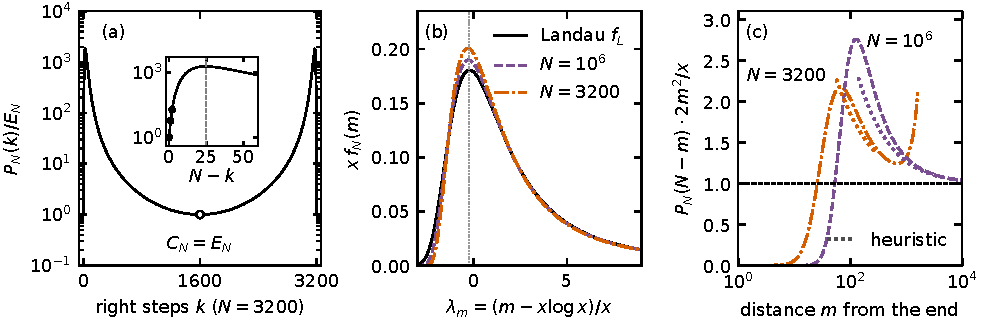
\includegraphics[width=\textwidth]{figures/Fig2}
\caption{The elephant walk at its crossing. (a) The law $P_N$ for $N=3200$
at its crossing $x=11.5468$, divided by the end $E_N$. The center equals the end,
and the law rises from each end to a mode and falls to the center. The inset
shows the last 60 values, with dots at $N$, $N-1$ and $N-2$. The end is
below its neighbor, and the modes are at distance 25 from each end (dashed). (b) The
law of $M_N$, scaled as $xf_N(m)$, against $\lambda_m=(m-x\log x)/x$, with the
Landau density $f_L$. The dotted line is its mode $\lambda_{\mathrm L}$. (c) The tail
$P_N(N-m)$ divided by $x/(2m^2)$. The dashed line is the reference value $1$, and the dotted curves are the heuristic correction
$1+x(2\log m+2\gamma-3)/m$ for $2x\log x\le m\le N/x$. The rise of the
$N=3200$ curve near $m=N/2$ is the mirror term $f_N(N-m)$. At $N=10^6$ we use
$x=g_N=22.4407$.}
\label{fig:shape}
\end{figure}

\begin{theorem}[endpoint dip]\label{thm:dip}
Let $N\ge2$ and $0<\varepsilon<1$, and put $\rho_1=P_N(N-1)/E_N$. Then
\[
 \rho_1>\frac{x}{2(1-\varepsilon)}.
\]
If moreover $N\ge3$ and $\varepsilon\le\frac12$, then
\[
 \rho_1\le\frac{x(1+1/N)^2}{2-3\varepsilon}+\frac{\varepsilon}{1-\varepsilon}.
\]
Hence the end is strictly below its neighbor if $x\ge2(1-\varepsilon)$. If $N\ge3$,
$\varepsilon\le\frac12$ and the right side of the second bound is below $1$, the end is
strictly above its neighbor.
\end{theorem}

\begin{proof}
By Lemma~\ref{lem:erw-reduction}, $\rho_1=\bigl(f_N(1)+f_N(N-1)\bigr)/f_N(0)$
with $f_N(0)=(1-\varepsilon)^{N-1}$. We bound the two terms in turn.

\emph{The term $f_N(1)$.} On the event $M_N=1$ the chain moves up exactly
once, say from time $j-1$ to time $j$ with $2\le j\le N$. Before that it
stays at $0$ for $j-2$ steps, each with probability
$1-r_t(0)=1-\varepsilon$. The move up has probability $\varepsilon$. After it
the chain stays at $1$ at the times $k=j,\dots,N-1$, each with probability
$1-r_k(1)=(1-\varepsilon)(1-c'/k)$, where
$c'=(1-2\varepsilon)/(1-\varepsilon)\le1$. Multiplying and summing over
$j$ gives
\[
 f_N(1)=\varepsilon(1-\varepsilon)^{N-2}\sum_{j=2}^N\vartheta_j,\qquad
 \vartheta_j=\prod_{k=j}^{N-1}\Bigl(1-\frac{c'}k\Bigr).
\]
For the lower bound we use $c'\le1$. Then
$\vartheta_j\ge\prod_{k=j}^{N-1}(1-1/k)=(j-1)/(N-1)$, and these lower bounds sum to
$N/2$ over $2\le j\le N$. So $f_N(1)/f_N(0)\ge x/(2(1-\varepsilon))$. For
the upper bound let $N\ge3$ and $\varepsilon\le\frac12$, so that $c'\ge0$. Then
$1-c'/k\le e^{-c'/k}$ and $\sum_{k=j}^{N-1}1/k\ge\log(N/j)$
give $\vartheta_j\le(j/N)^{c'}$. As $(t/N)^{c'}$ is nondecreasing in $t$, we can compare
the sum with an integral, namely
\[
 \sum_{j=2}^N\vartheta_j\le\int_2^{N+1}\Bigl(\frac tN\Bigr)^{c'} dt
 \le\frac{N(1+1/N)^{c'+1}}{c'+1}\le\frac{N(1+1/N)^2(1-\varepsilon)}{2-3\varepsilon},
\]
using $c'\le1$ and $1/(c'+1)=(1-\varepsilon)/(2-3\varepsilon)$. So
$f_N(1)/f_N(0)\le x(1+1/N)^2/(2-3\varepsilon)$.

\emph{The term $f_N(N-1)$.} The event $M_N=N-1$ needs an up move at every
time. The first has probability $r_1(0)=\varepsilon$, and the one at time
$k\ge2$ has probability $r_k(k-1)=1-\varepsilon-(1-2\varepsilon)/k$. This lies
strictly between $0$ and $1$, as every $r_k(b)$ with $0<b<k$ does, and it lies in
$[\frac12,1-\varepsilon]$ when $\varepsilon\le\frac12$. So $f_N(N-1)>0$, and
$f_N(N-1)\le\varepsilon(1-\varepsilon)^{N-2}$ when $\varepsilon\le\frac12$. This makes
the lower bound strict and gives the term $\varepsilon/(1-\varepsilon)$ in the upper bound.
(For $N=2$ the values $1$ and $N-1$ coincide, and the argument is the same.)
\end{proof}

\begin{corollary}[the dip at the crossing]\label{cor:dip}
Let $N\ge2$ be even and $0<\varepsilon<1$, and suppose that $x\ge2(1-\varepsilon)$
and $C_N\le E_N$. Then $C_N\le E_N<P_N(N-1)$, and $P_N$ is not unimodal. In
particular, if $x_N\ge2(1-\varepsilon_N)$, then at the crossing $E_N=C_N<P_N(N-1)$, and
$P_N$ is not unimodal.
\end{corollary}

\begin{proof}
Theorem~\ref{thm:dip} gives $P_N(N-1)>E_N\ge C_N$. Suppose that $P_N$ is
nondecreasing on $\{0,\dots,k_0\}$ and nonincreasing on $\{k_0,\dots,N\}$.
It is symmetric about ${k_{\mathrm c}}$, so we may replace $k_0$ by $N-k_0$ and assume
$k_0\le {k_{\mathrm c}}$. Then $P_N(k)\le C_N$ for every $k\ge {k_{\mathrm c}}$, including $k=N-1$, which
is a contradiction.
\end{proof}

By Proposition~\ref{prop:mlr}, $C_N\le E_N$ holds exactly when
$\varepsilon\le\varepsilon_N$, and $x\ge2(1-\varepsilon)$ says that
$\varepsilon\ge2/(N+2)$. So the corollary covers the $\varepsilon$ with
$2/(N+2)\le\varepsilon\le\varepsilon_N$. In particular the condition
$x_N\ge2(1-\varepsilon_N)$ says that
$\varepsilon_N\ge2/(N+2)$. By Proposition~\ref{prop:mlr} it holds exactly
when $C_N\le E_N$ at $\varepsilon=2/(N+2)$. We now show that this is so for
every even $N\ge8$.

\begin{proposition}[the endpoint dip for $N\ge8$, computer-assisted]\label{prop:dip-hyp}
For every even $N\ge8$ we have $C_N<E_N$ at $\varepsilon=2/(N+2)$, and hence
$x_N>2(1-\varepsilon_N)$. So for every even $N\ge8$, at the crossing
$E_N=C_N<P_N(N-1)$, and $P_N$ is not unimodal. For $N=2$, $4$ and $6$ the
condition $x_N\ge2(1-\varepsilon_N)$ fails, and no $\varepsilon$ meets the hypotheses of
Corollary~\ref{cor:dip}.
\end{proposition}

\begin{proof}
\emph{The range $N\ge1688$.} Take $\varepsilon=2/N$. Then
$\varepsilon(1+\log N)\le\frac1{100}$, so Theorem~\ref{thm:erw-bounds}(b)
gives $C_N\le\frac8{N(N+2)}N^{4/N}e^{10400/N}$. The right side decreases in
$N$ and is below $1.4\cdot10^{-3}$ at $N=1688$. Since $\log(1-y)\ge-y-y^2$
for $0\le y\le\frac12$, we also have
$E_N=\frac12(1-\frac2N)^{N-1}\ge\frac12e^{-2-2/N}>0.06$. So $C_N<E_N$ at
$\varepsilon=2/N$, and Proposition~\ref{prop:mlr} gives $\varepsilon_N>2/N$.
Hence $C_N<E_N$ at $\varepsilon=2/(N+2)$ as well.

\emph{The range $8\le N<1688$.} For $N=8$ the ratio $C_N/E_N$ at
$\varepsilon=2/(N+2)$ is exactly $\frac{67903}{71680}<1$. For even
$10\le N\le2000$ the script \texttt{certify\_center.py} encloses
$\varepsilon_N$ in an interval, by computing $C_N-E_N$ in ball arithmetic at
its two ends and using Proposition~\ref{prop:mlr}, and it checks by an exact rational
comparison that the lower end of the enclosure lies above $2/(N+2)$. So
$\varepsilon_N>2/(N+2)$, and Proposition~\ref{prop:mlr} gives $C_N<E_N$ at
$\varepsilon=2/(N+2)$. The ratio of the lower end to $2/(N+2)$ is at least
$1.107$, with its minimum at $N=10$.

\emph{The three smallest $N$.} At $\varepsilon=2/(N+2)$ the ratio $C_N/E_N$ is
exactly $2$, $\frac53$ and $\frac{508}{405}$ for $N=2$, $4$ and $6$, so
$\varepsilon_N<2/(N+2)$ there. These ratios and the one for $N=8$ are computed
in exact rational arithmetic by \texttt{certify\_elephant.py}. The last claim of the proposition about
$N\ge8$ is Corollary~\ref{cor:dip}.
\end{proof}

\subsection{Compound Poisson and Landau approximations}

Every step that disagrees with $X_1$ belongs to a flipped family.
Recall the compound Poisson law $\CP_N$ from Section~\ref{sec:rare-results}.
The expected number of flipped vertices with a family of size $d$
is $x/(d(d+1))$. If no flipped step has a flipped descendant (as is
likely when $x^2\log N/N$ is small), then $M_N$ is exactly the sum
of the flipped family sizes. We approximate this sum by independent
Poisson family counts.

The compound Poisson law and its Landau limit are known
(Section~\ref{sec:prior}). Here we bound the total variation and local
errors explicitly, keeping the jump cutoff at $N-1$ in the local bound.
K\"olbig and Schorr~\cite{ks1984} compute $f_L$ and its mode.
Lemma~\ref{lem:landau-mode} gives a certified enclosure of the mode.

\begin{theorem}[compound Poisson approximation]\label{thm:cp}
For $N\ge1$ and $0<\varepsilon<1$,
\[
 \operatorname{TV}(f_N,\CP_N)\le\delta_\Sigma
 :=\varepsilon^2(NH_N-2N+1)+2\varepsilon^2(N-1)+4\varepsilon^2\sum_{k=0}^{N-2}(H_k^2+H_k).
\]
Also $\delta_\Sigma\le\delta_B
 :=\frac{x^2\log N}{N}+\frac{4x^2}{N}e^{4x^2/N}+\frac{4x^2(H_N^2+H_N)}{N}$.
\end{theorem}

Here $\operatorname{TV}(P,Q)=\frac12\sum_k|P(k)-Q(k)|$, so the bound
holds for every mass and event, and $\delta_\Sigma=O(x^2\log^2N/N)$.
Appendix~\ref{app:bulk-cp} couples marks with Poisson variables and
reveals parents successively. Changing one parent affects family sizes
along only two root paths, whose depth second moments have order $\log^2N$.

Families of size up to $x$ contribute nearly $x\log x$. Those of order $x$ give fluctuations of order $x$. Centering $M_N$ at $x\log x$ and
dividing by $x$ gives $\lambda_m$ and the index-one stable density $f_L$.
Appendix~\ref{app:bulk} shows that $e^{\Psi_{\mathrm L}}$ is the characteristic function
of a law of class $L$, so $f_L$ is unimodal by~\cite{yamazato1978}.

\begin{theorem}[Landau limit]\label{thm:landau}
\begin{enumerate}[(a)]
\item Let $x\ge1$ and $N\ge4x$. For every integer $m$, with $\CP_N(m)=0$ for $m<0$,
\[
 \bigl\lvert x\,\CP_N(m)-f_L(\lambda_m)\bigr\rvert\le E_0:=\frac{47+10.4\log x}x+\frac{2.7\,x}N
 \le47\Bigl(\frac{1+\log x}x+\frac xN\Bigr).
\]
\item Let $0<\varepsilon\le\frac14$ and $x\ge1$. For every integer $m\ge0$,
\[
 \bigl\lvert xf_N(m)-f_L(\lambda_m)\bigr\rvert\le E_0+x\delta_\Sigma
 \le47\Bigl(\frac{1+\log x}x+\frac xN\Bigr)+x\delta_B .
\]
\item Let $N_n\ge1$ and $0<\varepsilon_n<1$ for $n\ge1$, and put $x_n=N_n\varepsilon_n$. If
$x_n\to\infty$ and $x_n^2\log^2N_n/N_n\to0$, then $(M_{N_n}-x_n\log x_n)/x_n$ converges in
law to the law with density $f_L$.
\end{enumerate}
\end{theorem}

At the crossing, the disagreement count is about $x\log x$, with Landau fluctuations of order $x$ (Figure~\ref{fig:shape}(b)). Theorem~\ref{thm:erw-crossing} supplies both conditions of (c).
For the untruncated law, (c) is Pakes' theorem~\cite[p.~993]{pakes1993}.
Bertoin proves an analogue for vertices cut from a random recursive
tree's root in another regime~\cite[Proposition~1]{bertoin2014ejp}.
The contribution in (c) is the transfer to the walk. We know no earlier form of (a) or (b).

Appendix~\ref{app:bulk} proves the local bound by expanding the compound
Poisson exponent at zero and applying Fourier inversion. The expansion
gives the centering $x\log x$, and its remainder gives the rate.

To locate the modes we need to know that $f_L$ is curved at its maximum.

\begin{lemma}[the Landau mode]\label{lem:landau-mode}
\begin{enumerate}[(a)]
\item The unique mode $\lambda_{\mathrm L}$ of $f_L$ satisfies
\[
 -0.22278299<\lambda_{\mathrm L}<-0.22278297.
\]
The density is nondecreasing on
$(-\infty,\lambda_{\mathrm L}]$ and nonincreasing on $[\lambda_{\mathrm L},\infty)$.
\item The derivative vanishes at the mode, $f_L'(\lambda_{\mathrm L})=0$, and
$-0.0792\le f_L''(\lambda)\le-0.0786$ for
$-0.2229\le\lambda\le-0.2227$.
\item For every real $\lambda$,
$f_L(\lambda_{\mathrm L})-f_L(\lambda)\ge\Delta_L\min\{1,(\lambda-\lambda_{\mathrm L})^2\}$ with
$\Delta_L=1/50$.
\end{enumerate}
\end{lemma}

Appendix~\ref{app:bulk-mode} proves the lemma. Parts (a) and (b) also
have a Lean proof from class-$L$ unimodality. The constant in (c) uses
a finite ball-arithmetic cover. Lean checks the deduction from the
cover's gap bounds and unimodality (Appendix~\ref{app:data}).

\begin{corollary}[mode locations]\label{cor:mode-location}
\begin{enumerate}[(a)]
\item Assume~\eqref{eq:H} and use $\Delta_L$ from
Lemma~\ref{lem:landau-mode}(c). Let
$E_1=E_0+x\delta_B$ be the bound of
Theorem~\ref{thm:landau}(b), and put
\[
 E'=E_1+\frac{16x^2H_N}{N^2}+\frac{\lVert f_L''\rVert_\infty}{8x^2}.
\]
If $E'<\Delta_L/2$ and $m_{\max}\le N/4$, then every mode $\kappa_N\ge N/2$ of $P_N$
satisfies $\lvert m_N-x\log x-\lambda_{\mathrm L}x\rvert\le x\sqrt{2E'/\Delta_L}$,
and so does every mode of $f_N$.
\item For all sufficiently large $N$, even or odd, and every
$\varepsilon$ with $\log N\le x\le2\log N$, every mode $\kappa_N\ge N/2$ of $P_N$ has
\[
 \bigl\lvert m_N-x\log x-\lambda_{\mathrm L}x\bigr\rvert\le50\sqrt{x\log x},
\]
and so has every mode of $f_N$ in place of $m_N$. In particular this holds at the crossing,
with $x=x_N$, for every large even $N$ (Theorem~\ref{thm:erw-crossing}(b)).
\end{enumerate}
In (a) every constant is explicit. (Here
$\lVert f_L''\rVert_\infty\le16/\pi^4$, since the characteristic function
of $f_L$ has modulus $e^{-\pi\lvert t\rvert/2}$.)
Remark~\ref{rem:bulk} gives an explicit threshold for (b).
\end{corollary}

\begin{corollary}[a wider rare-reversal range]\label{cor:wider-mode-range}
Suppose $x\to\infty$ and $x^3\log^2N/N\to0$. For every mode
$\kappa_N\ge N/2$ of $P_N$, and every mode $m$ of $f_N$,
\[
 N-\kappa_N=x\log x+\lambda_{\mathrm L}x+o(x),\qquad
 m=x\log x+\lambda_{\mathrm L}x+o(x).
\]
Each error is
$O\bigl(\sqrt{x(1+\log x)}+x^{5/2}\log N/\sqrt N\bigr)$.
\end{corollary}

\begin{proof}
The hypotheses give $E'\to0$ in Corollary~\ref{cor:mode-location}(a).
They also give $\varepsilon\log N\to0$ and
$x\log^2(x+1)=o(N)$, so Lemma~\ref{lem:B-mode} puts $m_{\max}\le N/4$
eventually. That corollary applies, with
\[
 E'=O\left(\frac{1+\log x}{x}+\frac{x^3\log^2N}{N}\right).
\]
Taking the square root gives both error bounds.
\end{proof}

So each hump of the law at the crossing sits about
$x\log x-0.2228\,x$ steps from its end. The proof is in
Appendix~\ref{app:bulk-cor}. It compares $f_N$ at a mode with $f_N$ at the
integer nearest to $x\log x+\lambda_{\mathrm L}x$, and uses
Theorem~\ref{thm:landau}(b) and Lemma~\ref{lem:landau-mode}(c).

\begin{remark}[size of the approximation error]\label{rem:bulk}
The bounds of this subsection are far from sharp at the sizes we can
compute. At $N=10^6$ and $x=22.4407$ the bound $\delta_B$ is still about
$0.46$, but there the computed law has
$\lvert f_N(m)/\CP_N(m)-1\rvert\le3.6\cdot10^{-4}$ for $1\le m\le10^4$. At
every crossing we tested, $m_N$ equals the mode of $\CP_N$.
We certify the global gap $\Delta_L=0.02$, but the local bound needs
such a large $x$ that Corollary~\ref{cor:mode-location}(b) only gives
the impractical threshold $N_2=\lceil e^{30000}\rceil$.
The approximation errors above were computed in double precision and
are not used in the proofs.
\end{remark}
